\section{Introduction}

Agentic reinforcement learning (RL) has demonstrated significant performance improvements in handling complex real-world problems such as AI coding~\citep{le2022coderl,dou2024stepcoder}, deep search~\citep{zheng2025deepresearcher,qi2025webrl}, and embodied AI~\citep{zitkovich2023rt, wang2023voyager}.
Unlike traditional large language models (LLMs) that rely solely on internal knowledge, agents actively interact with real-world environments through external tools, such as shell commands, APIs, or device operations~\citep{cao2025skyrl}.
To enable these capabilities, agentic RL has become a critical component of the post-training pipeline and an important workload in cloud clusters~\citep{xiao2026mimo}.

\begin{figure}[t]

    \centerline{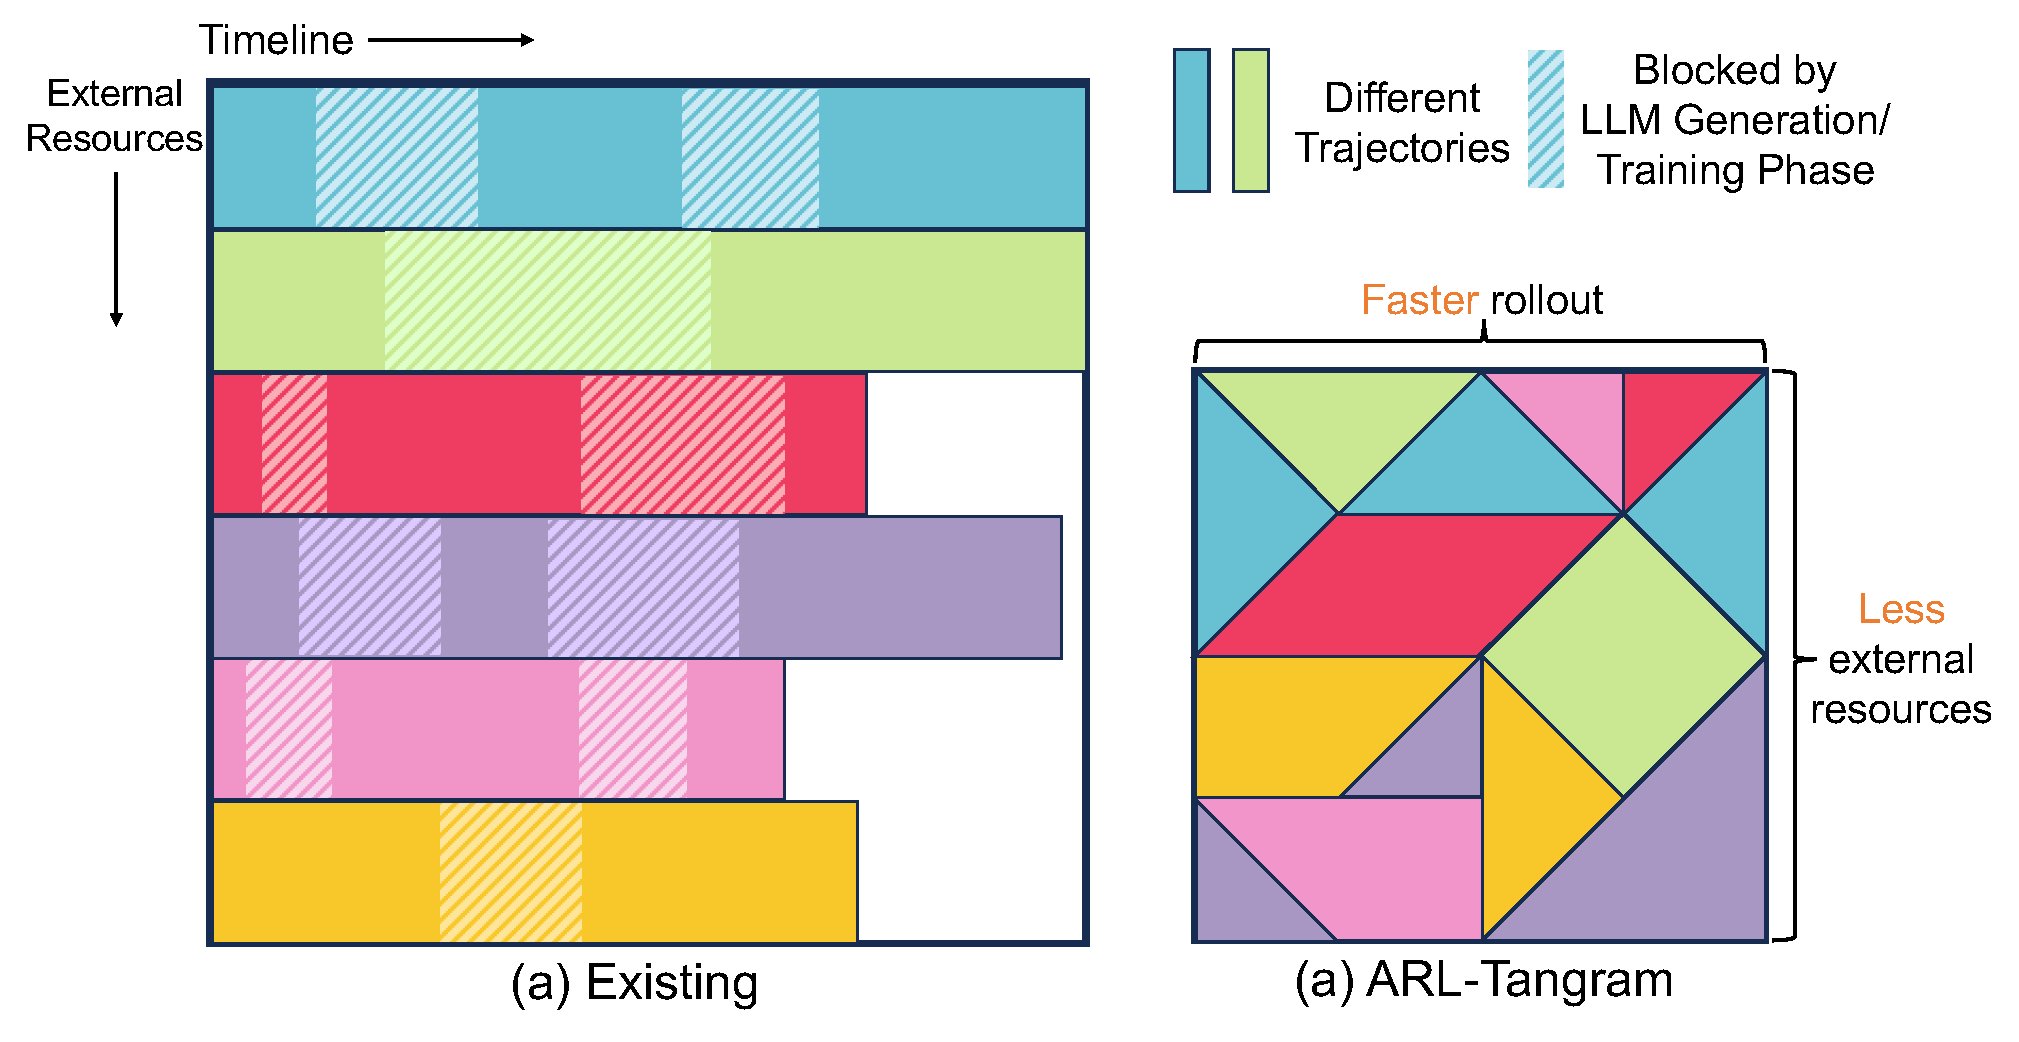
\includegraphics[width=0.9\linewidth]{figures/tangram.pdf}}
    \vspace{-0.2in}
    \caption{Comparison of existing approaches and \sysname. \protect\footnotemark}
    
    
    \label{fig:intro_op}
    \vspace{-0.2in}
\end{figure}


Unlike traditional RL, agentic RL demands substantial external resources, e.g., CPUs for AI coding, GPUs for reward models, and API quotas for web browsing.
These external resources, outside the primary training cluster, introduce additional management requirements.
Although this caters to the management approaches of cloud resources, the agentic scenario proposes higher demands for efficient management of these external resources, paramount for two reasons.
First, the latency of invocations is tightly coupled with the RL efficiency.
Without effective external resource management, invocations can become slow or even blocked, hindering the training speed, and even causing the entire training process to fail.
Second, the additional cost of external resources is non-negligible.
Agentic RL typically exhibits bursty invocation patterns, which requires provisioning numerous resources to maintain low invocation latency.
Thus, improving the utilization of these external resources and reducing the associated cost is undoubtably important.


\footnotetext{This is only a diagram for the insight of ARL-Tangram, where the patterns are not strictly triangles in practice.}

However, existing RL frameworks~\citep{sheng2025hybridflow,fu2025areal} often overlook the interdependencies between RL training and external resource usage.
These frameworks default to static resource-provisioning that leads to severe waste and inefficiency of external resources.
The over-provisioning exists at two levels (Figure~\ref{fig:intro_op}):
(1) At the trajectory level, systems often reserve dedicated resources, for the entire lifecycle of a trajectory, even though they are only invoked sporadically.
For example, in AI coding, the environment is accessed only for 47\% of its lifetime on average and leaving the allocated CPUs wasted for the remaining time.
(2) At the RL task level, tasks usually require specific external services and these services are deployed on isolated resources~\citep{jiang2025verltool,micromulti}.
However, due to the fluctuant pattern of external invocations, these resources are under-utilized and wasted.
In conclusion, previous static management limits system concurrency, leading to queuing delays and slower RL training.
% usually access different services and external resources are typically provisioned by services, preventing multiplexing even when sharing identical resource types.
% The phase alternation between rollout and training causes provisioned resources to sit idle during training phases.

% To address these inefficiencies, we propose \sysname, a unified action-level resource management system that decouples external resource management from the primary RL training cluster. 
% \sysname shifts the granularity of resource control from long-lived trajectories to individual atomic interactions, defined as "actions".
% By serving as a centralized intermediary between diverse RL tasks and a shared resource pool, \sysname enables statistical multiplexing across concurrent experiments and mitigates the resource idle time caused by long inactive agent environments.

% To address these inefficiencies, we propose the \textbf{action-level} scheduling that decouples external resource management from long-lived environments within trajectories or services within RL tasks.
% By \textbf{Breakdown}-ing the resource occupation of long-lived environments/services and \textbf{Pool}-ing the resources for invocations with the same resource type, we shift the granularity of resource control from original trajectory- or task-level into the level of atomic invocations, defined as "actions" in this paper. In addition, fine-grained resource management allows for elastic resource allocation to reduce the execution latency of actions.

To address these inefficiencies, we propose the \textbf{action-level} scheduling that shifts the granularity of external resource management from original trajectory- or task-level into a finer-grained action level, i.e., the level of atomic invocations.
We \textbf{breakdown} the resource occupation of long-lived environments/services and \textbf{pool} the resources for actions with the same resource type.
In addition, our fine-grained resource management allows for elastic resource allocation to reduce the execution latency of actions. 
As illustrated in Figure~\ref{fig:intro_op}, there are two RL tasks and 4 trajectories that invoke external resources of the same type, and the action-level scheduling enables less external resources by mitigating the over-provisioning and faster rollout by elastic resource allocation, compared with existing approaches.

However, realizing the action-level scheduling is non-trivial mainly because of three reasons. 
First, orchestrating actions with various external resources is complex.
Individual actions may exhibit requirements for multiple resource types, which is further complicated by varying elasticity and execution patterns of individual actions.
This necessitates a generalized abstraction model.
Second, the scheduler must operate subject to latency-sensitive workloads.
Action durations may be only microseconds, leaving an extremely short window for scheduling decisions.
This requires a lightweight algorithm capable of handling high-concurrency and bursty workloads.
Finally, how to uniformly and efficiently manage heterogeneous external resources with diverse characteristics and topologies is also challenging.
%action-level scheduling requires decoupling resource allocation from long-lived stateful agent environments.\zhl{what does this mean?}
% \sysname must release resources after each atomic action while preserving the environment state to ensure fast restoration, a direct conflict with traditional persistent allocation models.
% The system should be able to provide reliable resource sharing (which can release resources after each action while preserving the environment state), and low-overhead elasticity (which can deploy services with different parallelism fast).

Therefore, we design \sysname (\textbf{A}gentic \textbf{R}einforcement \textbf{L}earning \textbf{Tangram}), an action-level resource management system to uniformly orchestrate all these external resource invocations.
First, it utilizes a unified action formulation to manage actions with heterogeneous resource requirements and costs.
% heterogeneity, instead of treating actions as invocations that heterogeneous in costs and static in execution.
It formulates every action with a vectorized resource cost that accounts for various constraints, including CPU, GPU, memory, and API quotas.
Crucially, this formulation incorporates elasticity modeling, allowing the system to distinguish elastic actions and calculate the reduction in execution durations when allocating more resources.
This formulation enables \sysname to normalize various types of actions into a common format for scheduling.

The core of \sysname is an elastic resource scheduling algorithm designed to minimize the action completion time (ACT).
% \xbj{rewrite below}
Recognizing that shorter execution duration of actions improves the end-to-end efficiency of agentic RL training, 
we propose a heuristic scheduling algorithm, with a greedy eviction mechanism, to orchestrate actions based on the formulation and real-time system states. %, while maintaining low scheduling overhead.
The greedy eviction dynamically determines the scheduling strategies, avoiding overly aggressive/conservative allocation that lead to suboptimal ACT and degraded RL efficiency. %, while the entire scheduling algorithm is designed for actions with various invocation patterns.
% For practical usage, our scheduling algorithm maintains low overhead and is general for various action patterns.
% the scheduler dynamically performs resource allocation for each action, based on the formulation of actions and real-time system states.

% With these elastic scheduling decisions, 
\sysname tailors resource managers for heterogeneous resources, each with the specialized mechanism to efficiently \textbf{breakdown}, i.e., release the resources after each action and restore the states of environments or services when invoked, and effectively \textbf{pool}, i.e., allocate resources in the principle of mitigating fragmentation and improving parallel efficiency. 
Despite heterogeneous characteristics and topologies of resources, these managers expose a standardized interface to the scheduler, maintaining transparency of heterogeneous resources to the scheduling algorithm.
% The managers orchestrate actions of heterogeneous resources while maintaining the transparency in terms of the unified scheduler.

We implement \sysname as a standalone system regardless of the RL framework, external invocation types, and external resource types.
This design choice provides generality and simplicity to run with different external resources and across different RL frameworks.
We evaluate \sysname on real-world agentic RL training tasks, and the experimental results show that \sysname improves average ACT by up to 4.3$\times$, speeds up the step duration of RL training by up to 1.5$\times$, and saves external resources by up to 71.2$\%$. This system has been deployed to support the RL training of the MiMo series models.

In summary, this paper makes the following contributions,
\begin{itemize}[leftmargin=10pt]
% \vspace{-0.1in}
    \item We analyze the critical problem of external resource over-provisioning in agentic RL training, categorizing it into over-provisioning within trajectories and within RL tasks.
    \item We propose the action-level scheduling, and incorporates it into \sysname, a unified resource management system that shifts management from trajectory-level to action-level and enables fine-grained resource sharing and elasticity.
    \item We design a unified action formulation along with an elastic scheduling algorithm that minimizes ACT while respecting heterogeneous constraints. Besides, heterogeneous resource-specific managers further improve external resource utilization and training efficiency.
    \item We evaluate \sysname with real RL training tasks, showing that it significantly improves the end-to-end efficiency of agentic RL training and reduces external resource cost.

\end{itemize}


    % \item recognize and point out the critical issue during agentic RL training, over-provisioning of external resources